%%%%%%%%%%%% INTRODUCCIÓN  %%%%%%%%%%%%

\begin{center}
	{\fboxrule=4pt \fbox{\fboxrule=1pt
		\fbox{\LARGE{\bfseries 1. Introducción}}}} \\
	\addcontentsline{toc}{chapter}{1. Introducción}
	\setcounter{chapter}{1}
	\setcounter{section}{0}
	\rule{15cm}{0pt} \\
\end{center}

\pagenumbering{roman}
 
 \lettrine[lines=3, depth = 0]{E}{n} este documento explicar\'e c\'omo he llevado a cabo la práctica 1 de la asignatura \textbf{Sistemas Inteligentes} que consiste 
 en realizar un análisis de un Sistema Basado en Algoritmo Genético (\texttt{AG}) siguiendo las especificaciones indicadas en el gui\'on del proyecto.
 \par Un Algoritmo Genético (\texttt{AG}) es una variante de la búsqueda de haz estocástica, que a su vez es análoga a la ascensión de colinas estocástica, en la que los estados sucesores se generan combinando dos estados padres, 
 más que modificar un solo estado. 
 \par La búsqueda de haz estocástica muestra algún parecido con el proceso de selección natural, 
 por lo cual los <<sucesores>> (descendientes) de un <<estado>> (organismo) pueblan la siguiente generación según su <<valor>> (idoneidad o salud).
 La analogía a la selección natural es la misma que con la búsqueda de haz estocástica, excepto que ahora tratamos 
 con reproducción sexual más que con la reproducción asexual.

%%% IMAGEN DE SBR %%%
\begin{figure}[H]
	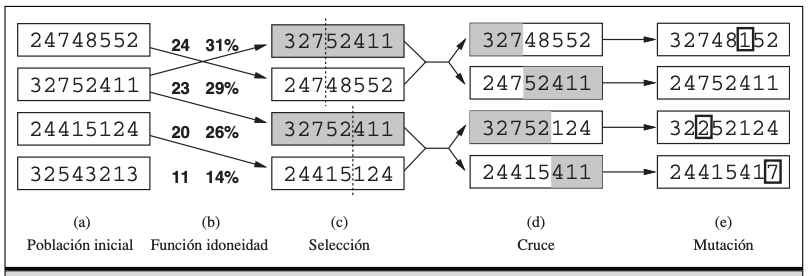
\includegraphics[width=\textwidth]{AG}
	\centering
	\caption{\textbf{Algoritmo genético.} La población inicial en (a) es ordenada con la función idoneidad en (b), y resultan pares para acoplamiento en (c). 
	Ellos producen los descendientes en (d), que están sujetos a mutación en (e).}
    	\label{fig:AG}
\end{figure}
 
\section{Elementos de un AG}
	\subsection{Codificación}
	\par Los \texttt{AGs} comienzan con un conjunto de \texttt{k} estados generados aletaoriamente, llamados población. 
	La codificación define el tamaño del espacio de búsqueda y el tipo de operadores. La información de cada
	estado se codifica en una cadena que llamamos cromosoma o genotipo. 
	Cada estado, individuo o fenotipo, está representado como una cadena sobre un alfabeto finito. 
	\newpage
	\begin{itemize}
		\item \textbf{Codificación binaria}: son cadenas de 0s y 1s.
		\item \textbf{Codificación entera}: se suele utilizar para problemas de localización.
		\item \textbf{Codificación de orden}: los individuos se representan como permutaciones, se suele utilizar para problemas de secuenciación.
		\item \textbf{Codificación real}: es una forma natural de codificar la solución, utilizando valores reales como genes.
	\end{itemize}
	Por ejemplo, un estado de las ocho reinas debe especificar las posiciones de las ocho reinas, cada una en una columna de ocho 
	cuadrados, y se requieren $8 \cdot log_2 8 = 24 bits$. O bien, el estado podría representarse como ocho dígitos, cada uno en el rango 
	de uno a ocho. La Figura \ref{fig:AG}(a) muestra una población de cuatro cadenas de ocho dígitos que representan estados de ocho reinas.
	
	\subsection{Función idoneidad}
	\par El valor heurístico de un estado es denominado fitness o idoneidad. La función fitness mide la calidad, respecto a alguna 
	característica, de los estados.
	\par En la Figura \ref{fig:AG}(b) cada estado se tasa con la función de evaluación o (en terminología AG) la función idoneidad. 
	Una función de idoneidad debería devolver valores más altos para estados mejores, así que, para el problema de las 8-reinas 
	utilizaremos el número de pares de reinas no atacadas, que tiene un valor de 28 para una solución. Los valores de los cuatro 
	estados son 24, 23, 20 y 11. En esta variante particular del algoritmo genético, la probabilidad de ser elegido para la reproducción
	 es directamente proporcional al resultado de idoneidad, y los porcentajes se muestran junto a los tanteos.

	\subsection{Operadores genéticos}
	\par El \texttt{AG} dispone de 3 operadores genéticos básicos, que son dependientes del tipo de codificación utilizada.
	\begin{itemize}
		\item \textbf{Selección}: encargados de escoger qué individuos van a disponer de oportunidades de reproducirse y cuáles no. Habrá
		individuos que aparezcan más de una vez e individuos que no aparezcan.
		\par En la Figura \ref{fig:AG}(c), se seleccionan dos pares, de manera aleatoria, para la reproducción, de acuerdo con las probabilidades en \ref{fig:AG}(b). 
		Notemos que un individuo se selecciona dos veces y uno ninguna. Hay muchas variantes de esta regla de selección. Puede demostrarse que el método selectivo, 
		en el que se desechan todos los individuos debajo de un umbral dado, converge más rápido que la versión aleatoria.
		\par Para que cada par se aparee, se elige aleatoriamente un punto de cruce de las posiciones en la cadena. 
		Por ejemplo, en la Figura \ref{fig:AG} los puntos de cruce están después del tercer dígito en el primer par y 
		después del quinto dígito en el segundo par. Son aquí los asuntos de codificación. Si se usa una codificación de $24 bit$ en vez de ocho dígitos, 
		entonces el punto de cruce tiene $2/3$ de posibilidad de estar en medio de un dígito, que resulta en una mutación esencialmente 
		arbitraria de ese dígito.
		\item \textbf{Cruce}: los individuos seleccionados son recombinados para producir la descendencia que se insertará en la siguiente generación.
		\par En la Figura \ref{fig:AG}(d), los descendientes se crean cruzando las cadenas paternales en el punto de cruce.
		Por ejemplo, el primer hijo del primer par consigue los tres primeros dígitos del primer padre y los dígitos restantes del segundo 
		padre, mientras que el segundo hijo consigue los tres primeros dígitos del segundo padre y el resto del primer padre. 
		En la Figura \ref{fig:AG} se muestran los estados de las ocho reinas implicados en este paso de reproducción. 
		El ejemplo ilustra el hecho de que, cuando dos estados padres son bastante diferentes, la operación de cruce puede producir 
		un estado que está lejos de cualquiera de los estados padre. Esto es, a menudo, lo que ocurre al principio del proceso en el que 
		la población es bastante diversa, así que el cruce (como en el temple simulado) con frecuencia realiza pasos grandes, al principio, 
		en el espacio de estados en el proceso de búsqueda y pasos más pequeños, más tarde, cuando la mayor parte de individuos son bastante
		 similares.
		\item \textbf{Mutación}: la mutación provoca que algunos de los genes de un individuo varíe su valor.
		\par En \ref{fig:AG}(e), cada posición está sujeta a la mutación aleatoria con una pequeña probabilidad independiente. 
		Un dígito fue transformado en el primer, tercer, y cuarto descendiente. El problema de las 8-reinas corresponde a 
		escoger una reina aleatoriamente y moverla a un cuadrado aleatorio en su columna.
	\end{itemize}

\section{Proceso que sigue dicha técnica}
	
	\par Los algoritmos genéticos combinan una tendencia ascendente con exploración 
	aleatoria y cambian la información entre los hilos paralelos de búsqueda. La ventaja primera, si hay alguna, del algoritmo 
	genético viene de la operación de cruce. Aún puede demostrarse matemáticamente que, si las posiciones del código genético 
	se permutan al principio en un orden aleatorio, el cruce no comunica ninguna ventaja. Intuitivamente, la ventaja viene 
	de la capacidad del cruce para combinar bloques grandes de letras que han evolucionado independientemente para así realizar 
	funciones útiles, de modo que se aumente el nivel de granularidad en el que funciona la búsqueda. Por ejemplo, podría ser 
	que poner las tres primeras reinas en posiciones 2, 4 y 6, donde ellas no se atacan las unas a las otras, constituya un bloque 
	útil que pueda combinarse con otros bloques para construir una solución.

	\par La figura \ref{fig:pseudocodigo} describe un algoritmo que implementa todos los pasos descritos en las anteriores secciones.
	%%% IMAGEN DE SBR %%%
	 \begin{figure}[H]
		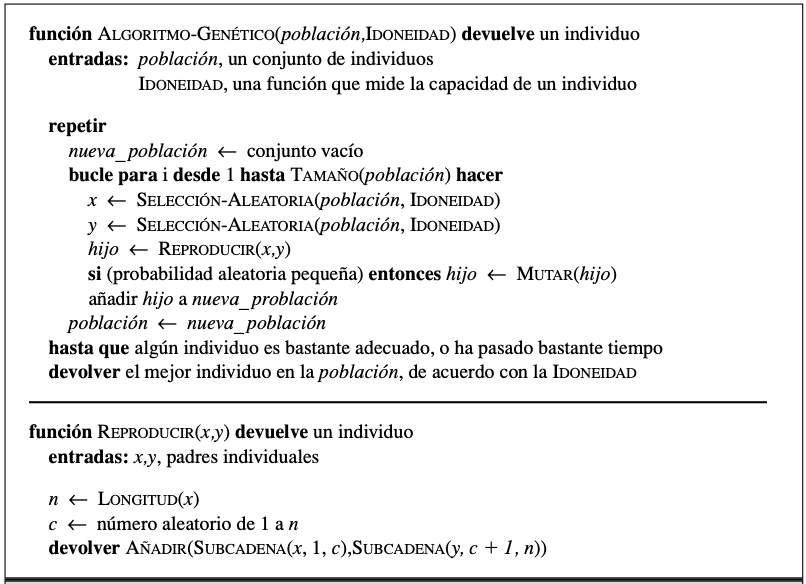
\includegraphics[width=\textwidth]{pseudocodigo}
		\centering
		\caption{\textbf{Algoritmo genético.} El algoritmo es el mismo que el de la Figura \ref{fig:AG}, 
		con una variación: es la versión más popular; cada cruce de dos padres produce sólo un descendiente, no dos.}
			\label{fig:pseudocodigo}
	\end{figure}
\newpage
\pagenumbering{arabic}